\documentclass[12pt,a4paper,oneside]{book}
\usepackage[french]{babel}
\usepackage[usenames,dvipsnames]{color}
\usepackage[utf8]{inputenc}
\usepackage{textcomp}
\usepackage[T1]{fontenc}
\usepackage{lmodern}	
\usepackage{bibunits} 
\usepackage{graphicx}
\usepackage{wrapfig}
\usepackage{glossaries}
\newacronym{w3c}{W3C}{World Wide Web Consortium}
\newacronym{rdf}{RDF}{Resource Description Framework}
\newacronym{trdf}{tRDF}{Temporal RDF}
\newacronym{strdf}{stRDF}{spatial and temporal Resource Description Framework}
\newacronym{lod}{LOD}{Linked Open Data}
\newacronym{sparql}{SPARQL}{SPARQL Protocol and RDF Query Language}
\newacronym{owl}{OWL}{Web Ontology Language}
\newacronym{stsparql}{stSPARQL}{spatial and temporal SPARQL Protocol and RDF Query Language}
\newacronym{uri}{URI}{Uniform Resource Identifier}
\newacronym{iri}{IRI}{Internationalized Resource Identifier }
\newacronym{sql}{SQL}{Structured Query Language}
\usepackage{float}
\usepackage{cite}
\usepackage{caption}
\usepackage{subcaption}
\usepackage{amsmath,mathtools}
\usepackage{subcaption}
\makeindex
\begin{document} 
\author{Moncef BEN RAJEB} 
\title{Annotation Temporelle Des Données DBpedia} 
\date{Juin 2014} 
\maketitle 
\frontmatter
\tableofcontents 
\addcontentsline{toc}{chapter}{Remerciement}
\addcontentsline{toc}{chapter}{Introduction générale}
\chapter*{Remerciements}
\paragraph{}
Avant de vous décrire ce que j’ai appris durant ma première expérience dans le milieu de recherche, il me semble opportun de commencer par des remerciements, à ceux qui m’ont appris durant ces quatres mois de stage. 
\subparagraph{}
Je tiens également à exprimer mes vifs remerciements à mes encadrants de stage {\it M. Antoine Zimmermann et Mme Mihaela Juganaru-Mathieu} pour l’aide déterminante qu’ils m’ont accordée, pour l’intérêt qu’ils ont apporté à mon travail et à mon apprentissage et pour m’avoir accompagné tout au long de cette expérience avec beaucoup de patience et de pédagogie.
\subparagraph{}
Je remercie particulièrement {\it Mme Mathieu et M. Valentin Brun} qui ont partagé leur bureau avec moi durant ce stage. 
Je remercie l'ensemble de l'équipe informatique de l'Institut Henri Fayol de m'avoir accueilli et de m'avoir
invité à participer à la vie de l'équipe.
\subparagraph{}
Enfin, je remercie tous mes professeurs de l’université de Jean Monnet et l'école des mines, ma famille, mes amis et toute personne qui s’intéresse au contenu de mon rapport.

\section*{Introduction générale}
\paragraph{}
Depuis la création du web il y a de cela vingt-cinq ans déjà, ce monde virtuel a vécu une évolution constante. Il offre une multitude de services aux utilisateurs individuels, aux entreprises, mais aussi à la société. Au fil des années, plusieurs versions du web ont vu le jour : le web documentaire, le web applicatif, le web social, le web mobile, etc...
\subparagraph{}
Dans le contexte de l’évolution du web une nouvelle version dite le web sémantique et sociale qui vise à propager nos modèles et leurs logiques; s’apprête à avoir le jour. Il y a plusieurs facettes du web, et le web sémantique offre un élément de réponse à l’intégration de chacune de ces facettes. Il propose d’utiliser des métadonnées pour annoter les ressources du web, et d’exploiter la sémantique des schémas de ces annotations pour les traiter avec intelligence.
\subparagraph{}
Le domaine du web sémantique est un objet de recherche sur les métadonnées du web. L'objectif principale de la naissance du web sémantique c'est d’en avoir une nouvelle version du web bien structurée qui soit capable d’en assurer le contrôle efficace des métadonnées. Dans ce contexte, DBpedia\footnote{http://dbpedia.org/About} est une base de donnée structurée qui contient des informations extraites de Wikipedia\footnote{http://wikipedia.org} et rend ces informations disponibles sur le web.
\subparagraph{}
Aussi, Resource Description Framework (RDF) est le premier des standards de la web sémantique et se trouve être un modèle à plusieurs syntaxes, dans une est  “Turtle”\footnote{http://www.w3.org/TeamSubmission/turtle/} pour publier des données à thèmes variés sur le web.
\subparagraph{}
Ce langage de modélisation permet à quiconque de décrire des ressources sur le web et aussi des ressources du web. Dans ce modèle connu comme étant la “lingua franca” du web, tout est exprimé sous forme de triplets $(subject, predicate, object)$ où chaque triplet contribue à une description du monde.
\paragraph{}
Néanmoins, des faits tels que ceux donnés dans DBpedia sont en mesure d’être adaptés au changement perpétuel du monde.
RDF n’est pas bien équipé pour exprimer d’une manière cohérente la validité temporelle des états, tels que “Obama est le président des États-Unis depuis 2008”. 
\subparagraph{}
Pour surmonter ce problème avec une modélisation RDF adéquate, plusieurs anciens travaux de recherches ont proposé d’attacher à ces triplets des annotations temporelles, ceci revient à une formalisation de ces états avec des contraintes temporelles comme des quadruplets de la manière suivante $(subject, perdicate, object, time)$ à la place du formalisme de triplet habituel.
\subparagraph{}
La théorie derrière un modèle de données basé sur des quadruplets évolue autour des termes de représentation, de connaissance, de raisonnement mais aussi d’interrogation. Or, le problème c’est qu’ils ne donnent aucune indication sur la façon dont les annotations temporelles sont créées.
\paragraph{}
De ce fait, l’objectif de ce stage est d’une part, l’extraction des informations temporelles depuis les différents documents en utilisant les techniques de fouille de données et d’autre part, d’annoter ces ressources selon leurs contextes, tout ceci mettre ces informations sous forme de quadruplets structurés dans BDpedia.
\newpage
\section*{Portée du document }
\paragraph{}
Ce mémoire de master résume les recherches, réflexions, modélisations, propositions et développements réalisés durant ce stage. Il conclut la seconde année de master Web Intelligence. Le contenu est organisé de la manière suivante :
\begin{itemize}
\item Une première partie présente l’état de l’art réalisé sur l’annotation temporelle des triplets RDF dans les bases de connaissances.
\item La deuxième partie englobe les diverses propositions pour répondre au besoins identifiés.
\item La troisième partie développe l’aspect technique de la mise en oeuvre.
\item La quatrième partie ouvre des perspectives.
\end{itemize}
\mainmatter 
\documentclass[12pt,a4	]{report}
\usepackage[frenchb]{babel}

\usepackage[usenames,dvipsnames]{color}
\usepackage[utf8]{inputenc}
\usepackage{textcomp}
\usepackage[T1]{fontenc}
\usepackage{lmodern}	
\usepackage{bibunits}
\usepackage{graphicx}
\usepackage{wrapfig}
\usepackage{glossaries}
\makeglossaries
\usepackage{float}
\usepackage{cite}
\usepackage{caption}
\usepackage{amsmath,mathtools}
\usepackage{subcaption}

\newacronym{w3c}{W3C}{World Wide Web Consortium}
\newacronym{rdf}{RDF}{Resource Description Framework}
\newacronym{strdf}{stRDF}{spatial and temporal Resource Description Framework}
\newacronym{lod}{LOD}{Linked Open Data, Web de données}
\newacronym{sparql}{SPARQL}{Protocol and RDF Query Language}
\newacronym{stsparql}{stSPARQL}{spatial and temporal Protocol and RDF Query Language}
\newacronym{uri}{URI}{Uniform Resource Identifier}
\newacronym{iri}{IRI}{Internationalized Resource Identifier }
\newacronym{sql}{SQL}{Structured Query Language}


\begin{document}


\section*{État de l'art}
\subsubsection*{Introduction}
\paragraph{}
Dans ce chapitre nous introduisons les différentes technologies qu'on va utiliser dans notre étude ainsi que les travaux de recherche liée à cette problématique; toute en essayant d'analyser les différentes approches. Afin de mettre en place la solution que nous avons proposé.  Nous aborderons ce dernier point dans le prochain chapitre.

\subsection*{Apperçu du domaine}
\paragraph{}
Notre étude a la particularité d’englober le domaine de la fouille de données et du Web sémantique. 
En effet, on utilise les techniques de la fouille pour l'extraction des données depuis les différentes sources d'informations, et le Web sémantique afin de donner au métadonnées une structure plus lisible par la machine.
\subparagraph{}
Dans ce chapitre on présente les téchnologies du Web sémantique que nous avons utilisé, puis nous effectuons une étude préliminère autour des travaux de recherche qui précède notre étude toute en introduisant les concepts et la problèmatique de notre sujet.
\subsection*{Technologies du Web sémantique}
\subsubsection*{Intérêt du Web sémantique}
\paragraph{}
Le Web sémantique est un domaine de recherche né des travaux de Tim Berners-Lee l'un des pionniers dans ce secteur~\cite{Berners-lee2001} dont le but était d'ajouter du sens aux contenus du Web. Ce n'est pas une question d'ajouter une autre alternative du Web mais c'est plustôt d'étendre le Web actuel dans le but d'utiliser et manipuler le maximum de son contenu informatiquement. En clair, c'est de permettre à des programmes informatiques de traiter un ensemble étendu de données issues du Web.
\subsubsection*{Modèle RDF}
\paragraph{}
Au centre du Web sémantique, comme la brique d’argile qui permet d’ériger les plus grands édifices, se trouve le modèle \gls{rdf} . RDF\footnote{http://www.w3.org/RDF/} est un standard de \gls{w3c}, il se base sur un modèle de graphe sous forme de triplets (sujet, prédicat, objet) qui permettent d'exprimer tous types d'assertions. Il s’agit d’un cadre de description de ressources, d’une façon formelle sur le Web.
C’est la première brique de standard du Web sémantique qui recouvre à la fois un modèle et plusieurs syntaxe pour publier des données variées sur le Web.
\subparagraph{}
Dans RDF ~:
\newline
\begin{itemize}
\item Les ressources sont un concept de base du Web sémantique, tout ce qui peut être référencé est une ressource. Dans un contexte plus technique~: on déduit que tout ce qui peut être identifié par un \gls{uri} / \gls{iri} peut être considéré comme ressource.
\item Un ensemble d’attributs décrivent la ressource, qui possèdent des caractéristiques et des relations avec d’autres ressources.
\item Le cadre standardise la syntaxe de ces descriptions, les modèles et les langages.
\end{itemize}
\subparagraph{}
La plus petite structure de description en RDF est le triplet.
\begin{figure}[H]
\centering
\centering
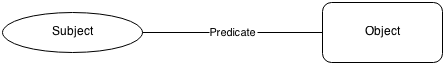
\includegraphics[width=8cm]{tripletrdf.png}
\caption{triplet RDF}

\end{figure}
\subparagraph{}
Un triplet décrit une ressource, l’associe à une propriété et une valeur de cette propriété qui peut être une nouvelle ressource liée.
\newline
Par exemple “Moncef a écrit une page QuadsRDF.html à propos des quadruplets RDF” peut être décomposée en deux triplets ayant comme sujet “QuadsRDF.html”: <QuadsRDF.html, auteur, Moncef> et <QuadsRDF.html, thème, quadruplets RDF>.
\newline
On peut schématiser cela de la manière suivante:
\begin{figure}[H]
\centering
\centering
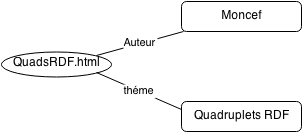
\includegraphics[width=8cm]{Diag.png}
\caption{Deux Triplets liés au même sujet}

\end{figure}
\subsubsection*{SPARQL}
\paragraph{}
Si RDF fournit un modèle universel de représentation de métadonnées. D'autres niveaux de traitements ont été standariser au dessus de lui et notament l'interrogation de ces métadonnées.
\gls{sparql} fournit le langage d'interrogation du Web sémantique, et en cela il est à RDF ce que \gls{sql} est au bases de données relationnelles.
\subparagraph{}
SPARQL est un langage d'interrogation de graphe RDF dont l'énoncé de base est lui aussi un triplet (ressource, propriété, valeur).Il est une recommandation du W3C depuis juillet 2008.
Poser une question en SPARQL consiste à écrire un graphe requête pour lequel on cherche des occurences dans le graphe cible.
\subsubsection*{N-Quads}
\paragraph{}
N-Triples est une simple syntaxe ligne délimitée( line-delimited) pour les graphes RDF. N-Quads\footnote{http://sw.deri.org/2008/07/n-quads/}, un format qui s'étend N-Triples avec le contexte. Chaque triplet dans un document N-Quads peut avoir une valeur de contexte en option:
\newline
<subjet> <prédicat> <objet> <contexte>.
\subparagraph{}
La notion de provenance est essentiel lors de l'intégration des données provenant de différentes sources ou sur le Web . Par conséquent, l'état de l'art des référentiels RDF (sujet, prédicat, objet, contexte) quadruplet, lorsque le contexte indique généralement la provenance d'une déclaration donnée.
\newpage
\subsection*{Base de Connaissances}
\subsubsection*{Introduction}
\paragraph{}
Une base de connaissance regroupe des informations spécifiques à un domaine donné, sous un format exploitable par un ordinateur. Elle peut contenir des régles, des faits ou d'autres représentations. Les base de connaissances regroupent des informations structurées et nous particulièrement on cherche à exploiter ces informations pour les mettres dans une nouvelle structure plus facilement exploitable par la machine.

\subsubsection*{DBpedia}
\paragraph{}

C'est un projet universitaire et communautaire d’extraction et d’exploitation automatique des données de wikipedia. C’est également un ensemble de données structurées et normalisées au format du Web sémantique.
\begin{wrapfigure}{r}{0.7\textwidth}
\vspace{-10pt}
\begin{center}
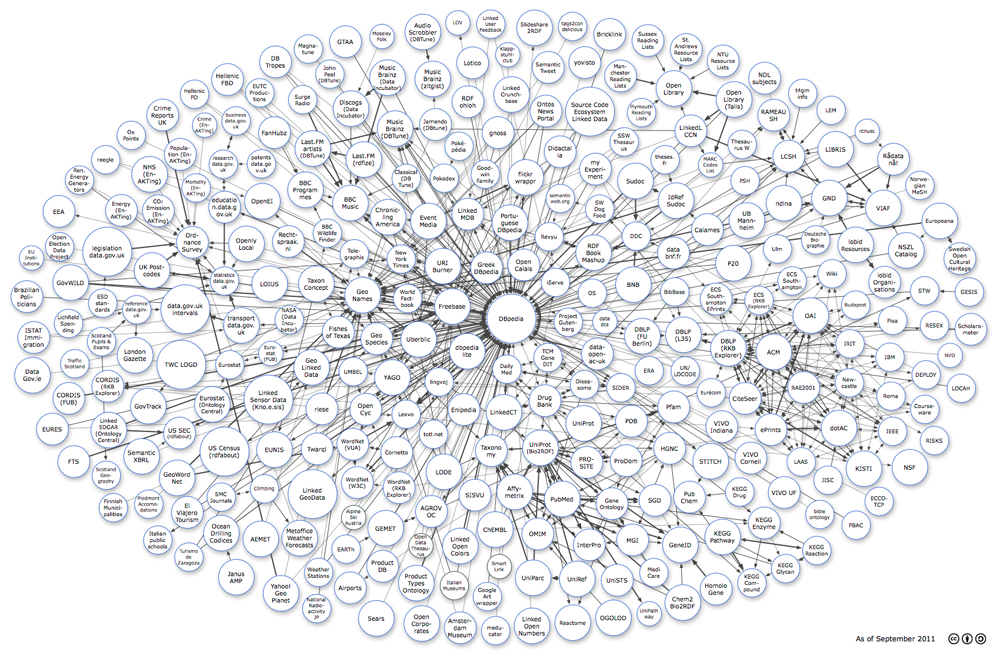
\includegraphics[width=0.50\textwidth]{dbpedia.png}
\end{center}
\vspace{-15pt}
\caption{DBpedia}
\vspace{-10pt}
\end{wrapfigure}
DBpedia 3.9 est la dernière version de DBpedia datant de Juin 2013.
\subparagraph{}
Cette base de connaissance est écrite en Scala et Java. Elle adopte les normes du Web sémantique et du réseau Linked Open Data. Pour chaque document encyclopédique, il existe une page de ressources contenant toutes les données sous forme de triplets RDF.
\newpage
\subsubsection*{YAGO}
YAGO\footnote{http://www.mpi-inf.mpg.de/yago-naga/yago/} est une large base de connaissance sémantique, délivré de Wikipedia, WordNet et GeoNames. Actuellement elle contient plus de 10 million entités (personnes, organisations, villes, etc..) et plus de 120 million faits de ces entités.
\newline
Les caractéristiques principales de YAGO :
\begin{itemize}
\item Une précision de 95\%, chaque relation est annoté avec sa valeur de confiance.
\item YAGO combine la taxonomie propre de WordNet avec la richesse du système de catégorie Wikipedia, l'attribution des entités à plus de 350 000 catégories.
\item YAGO est une une ontologie qui attache une dimension temporelle et spacial pour plusieurs de ces faits et entités.
\end{itemize}
\begin{figure}[H]
\centering
\centering
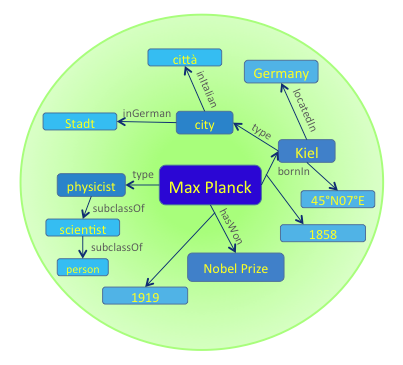
\includegraphics[width=11cm]{yago.png}
\caption{YAGO}

\end{figure}
\subsection*{Différentes approches d'annotation temporelle}			
\subsubsection{Introduction}
\paragraph{}
Dans le domaine du Web sémantique, il y a plusieurs extensions de RDF qui ont été proposé pour : la vérité, la confiance, la certitude, le temps ect…
Par exemple : Pour la verité de certaines triplets où le degré de la vérité est entre $0$ et $1$, l’instance “Rome is a big city to degree 0.8” peut être représentée par $(Rome, type,big{\_}city) : 0.8$.
\subparagraph{}
De même pour la certitude un autre forme a été proposé :
$(Max,hasSupervisor : (0.9,2003),William)$ à la forme générale suivante $(s, p : (x,t),o)$
\newline
La certitude $x$ est représentée sous forme d'un pourcentage, 90\% pour cet exemple.
\subsubsection*{L'annotation temporelle}
\paragraph{}
La nécessité de l’annotation temporelle sur les documents Web a été évoqué dans des nombreux travaux de recherche. La première approche formelle au problème de modélisation et d’interrogation temporelle en RDF a été introduite par Gutierrez et al~\cite{gutierrez2005}.
\subparagraph{}
Ensuite, Udrea et al~\cite{udrea2006} ont remis en question la notion d'annoter temporellement les graphes RDF et depuis plusieurs travaux de recherche ont évoqué cette problèmatique.
Ces derniers définissent le triplet annoté de la forme suivante $(s,p:t,o)$, $t$ est une étiquette temporelle.
De plus ils ont donné des algorithmes pour interroger les données RDF annotées.	

\subsection*{RDF Temporel ou tRDF}
\paragraph{}
Pour introduire RDF temporel ''tRDF'' on commence par les exemples suivants:
\newline
Il y a des triplets comme par exemple : " Mary est toujours la mère de John " qui n'ont pas une caractéristique temporelle explicite parce qu'il est toujours valide. Mais il y a aussi des triplets ayant une valeur vrai que dans une plage temporelle bien précise, par exemple : " Bill Clinton est le président de Etats Unis ", n'est valide que dans l'intervalle $[1993-2001]$.
\subparagraph{}
Donc il y a des triplets qui ne peuvent être reconnus que dans des périodes temporelles précises.
\paragraph{}
D'après Andrea et al~\cite{pugliese2008} l’annotation tRDF peut être exprimé de la manière suivante ($n$ est un nombre entier, $T$ appartient à un interval de temps, $s$ le sujet, $p$ le prédicat, $v$ l'objet) :
\begin{enumerate}
\item ($s$, $p$ : {$T$}, $v$), ce type de triplet représente une relation entre le sujet et le prédicat et l'objet dure un temps $T$ (dans n'importe quel point de temps dans $T$).
\item $($s$, $p$ : <$n$ : $T$>, $v$)$, ce triplet présente une relation entre $s$, $p$ et $v$ qui dure au moins n point de temps différents dans $T$.
\item ($s$, $p$ : [$n$ : $T$], $v$), ce triplet présente une relation entre $s$, $p$ et $v$ qui dure au plus $n$ points de temps différents dans $T$.
\end{enumerate}
\subsection*{L'importance de l'annotation temporelle dans LOD}
\subsubsection*{Présentation du LOD}
\paragraph{}
\gls{lod}\footnote{http://linkeddata.org/}, c'est un moyen de publier des données structurées sur le Web où les données contenues dans des bases de données sont exposées sur le Web avec leur sémantique, ce qui donne la possibilité au métadonnées d'être connectées et enrichies d'une manière solide, permet d'avoir plusieurs représentations d'un même contenu et fait des rapprochements entre des ressources connexes.
\subparagraph{}
Au cours des dernières années, le Web de donnée a développé dans une grande fusion de divers ensemble de données provenant de plusieurs domaines. Ce dernier décrit les ressources identifiées par des \gls{uri} en représentant leurs propriétés et des liens vers d’autres ressources. L'ensemble des données fournit des connaissances du monde réel.
\subsubsection*{Relation entre l'annotation temporelle et LOD}
\paragraph{}
Les informations sur un intervalle temporel de validité pour les évènements décrits par des triplets RDF jouent un rôle important dans un grand nombre d'applications.
Un grand nombre de triplets dans LOD ne sont valides que dans un certain intervalle de temps qu'ils l'appellent la protée de leurs temps.
Par exemple dans DBpedia ils indiquent que "Mario Balotelli joue pour les équipes AC Lumezzane et le Milan AC". Lorsqu'on modélise des connaissances du monde réel, Mario Balotelli ne peut pas jouer au même temps avec AC Lumezzane et le Milan AC.
\subparagraph{}
Les logiques temporelles d'informations ont besoin d'avoir de la protée temporelle des faits tels que “Mario Balotelli joue pour l'équipe AC Milan”.
Une approche a été proposée pour détecter la portée des évènements visés par des triplets RDF par Rule et al~\cite{rula2013}, elle se compose de quatre étapes principales~:
\begin{itemize}
\item Les données du document Web sont normalisées pour tenir compte de l’importance des dates figurants dans les documents.
\item La sortie de la phrase est comparée avec un ensemble d’intervalles de temps pertinents pour obtenir des notes de significations pour chaque intervalle.
\item Un ensemble d’intervalles plus importants est sélectionné.
\item Les intervalles sélectionnés sont fusionnés lorsque c’est possible.
\end{itemize}
\subparagraph{}
La plateforme DeFacto(Deep Fact Validation)~\cite{lehmann2012} a été utilisée pour la validation des états on cherchant des sources qu'elle confirme sur le Web.
\subparagraph{}
Les triplets sont représentés par des faits et peuvent être associé à un contexte temporelle.
Par exemple, $<Balotelli, team, AC Milan>$ se réfère à un événement de $2003-2009$, une annotation temporelle est rattachée au fait comme suit $<f, [ti,tj]>$.
\subparagraph{}
Cette approche combine deux types d'informations~: les informations temporelles recueillies dans des documents Web et les informations temporelles contenues dans les bases de connaissances, pour associer des intervalles de temps au triplets RDF.
\subsection*{Temps valide des triplets dans les données géospatiales liées}
\paragraph{}
Bereta et al~\cite{bereta2013} introduisent la composante temporelle des données du modèle stRDF et le langage de requêtes stSPARQL, récemment proposés pour la présentation et l’interrogation des données géospatiales liées qui changement dans le temps.
\subparagraph{}
L’introduction du temps dans les modèles de données et les langages de requêtes, a été l’objet de recherches approfondies dans le champs des bases de données relationnelles.
\subparagraph{}
Les trois types distincts de temps qui ont été étudiées~:
\begin{itemize}
\item L'action temporelle indépendante, par exemple ($01/12/1954$ c’est l’anniversaire de John).
\item Le temps d’évènement ou un fait vrai dans l’application (entre $2001-2012$ John a été professeur).
\item Le délail de transaction qui est le moment où un fait est en cours dans la base de données (l’heure système qui présente l’heure exact quand John est un professeur "$2001-2012$" est en cours dans la base de données).
\end{itemize}
\paragraph{}
Bereta et al~\cite{bereta2013} présentent également le concept de horodatages anonymes dans les graphes RDF, par exemple le quadruplet(quad) de la forme $(s, p, o)[t]$, où $t$ est une horloge ou un timestamp $x$ anonyme déclarant que le triplet est valable dans un certain point de temps inconnue.
\subparagraph{}
L’idée principale est d’intégrer les informations géospatiales pour le modèle de graphe RDF temporel. Le langage d’interrogation \gls{stsparql}\footnote{http://www.strabon.di.uoa.gr/stSPARQL}, ajoute deux nouveaux types de variables spatiales et temporelles, aux variables SPARQL standards.
\subsection*{Base de données temporelles}
\paragraph{}
Une base de données temporelle est une base de données avec des acpects de temps intégrés(temps-valide, temps-transaction), c'est à dire un modèle de données temporelles et une version temporelle du langage structuré de requête(SPARQL, SQL).
\subparagraph{}
En effet, le \textit{temps valide} dénote la période du temps durant laquelle un fait est vrai par rapport à la réalité.
Le \textit{temps-transaction} est la période de temps pendant laquelle un fait est stocké dans une base de données.
\paragraph{}
Dans le contexte de l'annotation temporelle des graphes RDF, les besoins se résume comme suit~:
\begin{itemize}
\item L'accès à des différents versions d’une ontologie.
\item Récupération des informations passées sur les sites Web.
\item La distribution des mise à jour des journaux.
\end{itemize}
\subparagraph{}
En vertu des travaux de Antoniou et al~\cite{antoniou2004} présentent une ontologie du service Web, pour monter qu'une ontologie peut passer par plusieurs états, ainsi que d'autres recherches dont l'objectif d'analyser et justifier les besoins cités auparavant.
\paragraph{}
Une base de données temporelle peut être exprimé comme un répertoire d'informations temporelles.
Gutiérrez et al~\cite{gutierrez2007}, montrent qu'il y aura deux manières pour ajouter des dimensions temporelles dans un graphe RDF intemporel~:
\begin{itemize}
\item Étiqueter les éléments soumis à des changements, les triplets par exemple, à chaque changement un nouveau graphe créer et l’ancien état sera stocké quelque part.
\item Versionner : capture de temps de transaction, l’étiquetage est mieux que les versions pour les raisons suivantes:
\begin{itemize}
\item Il conserve le principe de la nature distribuée et extensible de RDF.
\item Si la nouvelle version n’affecte que quelques éléments cela implique la création d’un nouveau graphe, de ce fait on aura des contraites de mémoire.
\end{itemize}
\end{itemize}
\paragraph{}
Gutiérrez et al~\cite{gutierrez2007}, ont travaillé sur le domaine temporel à base de points et ils ont aussi codé les points du temps en intervalle.
\subparagraph{}
Ces derniers ont proposé un vocabulaire pour affirmer les moments où les triplets sont valables dans un graphe RDF.
\subsection*{Graphe Temporel}
\paragraph{}
Un graphe temporel c'est des triplets$(s,p,o)$ avec des étiquettes temporelles qui représentent la période dans laquelle il est valable dans le monde réel.
Exemple le triplet $(s,p,o)$ est valable dans un temps $t$, $(a,b,c)[t]$, ou autrement dans un intervalle de temps $[t1,t2]$, $(a,b,c)[t1,t2]$.
\subparagraph{}
L'idée générale de Pugliese et al~\cite{pugliese2008} est d'annoter RDF avec un interval de temps.
Ces derniers ont proposé un graphe temporel d'indexation "tGRIN". C'est une structure d’indexation qui construit un index spécialisé pour RDF temporels qui sont stockés dans une base de données relationnelle "RDBMS".
\subparagraph{}
D’autres efforts pour stocker RDF dans une base relationnelles:
\begin{itemize}
\item Jena2 de Apache
\item Sesame de openRDF.org
\item 3store ou triplestore de University of Southampton
\end{itemize}
\paragraph{}
D'autes index temporels sont implémentés ( R+ trees, SR-trees, ST-index, and MAP21) mais l'index tGRIN présentent des performances supérieures selon les expérimentations faites dans~\cite{pugliese2008}.
\subsection*{Synthèse}
\paragraph{}
Plusieurs travaux de recherches on été mis au point pour résoudre le problème des données qui présentent un sémantique temporel dans les graphes RDF. Nous avons étudié ces travaux afin d'avoir une vision globale sur la problèmatique et pour voir ce qui est déjà fait dans ce domaine. On s'inspire de ces travaux pour proposer une nouvelle approche qui soit satisfaisante pour annoter temporellement les métadonnées de Wikipedia.
\subsection*{Extraction des données}
\subsubsection*{Introduction}
\paragraph{}
L'extraction, la fouille de données, ou encore la fouille des connaissances à partir de données, ont pour objet l'extraction d'un savoir, d'une connaissaince, ou dans notre cas une connaissance mise en relation temporelle à partir de grandes quantité de données par des méthodes automatiques.
\subsubsection*{Différentes approches de l'extraction }
\paragraph{}
Une approche proposée par Zweigenbaum et Tannier~\cite{zweigenbaum2013} consiste à détecter les relations temporelles entre les évènements et les expressions temporelles à partir des comptes rendu hospitaliers.
\subparagraph{}
La détection des relations temporelles entre les évènements dans un texte, fournit de bonnes informations pour l’extraction.
\newline
C’était les défis de TempEval Verhagen et al~\cite{verhagen2010} qui ont abordé en “domaine ouvert”, en cherchant à détecter en TempEval2 cinq types de relations temporelles :
\newline
$(Before, After, Overlap, Before\_or\_Overlap, Overlap\_or\_Before)$
et Identifier les relations temporelle décrivant la chronologie du séjour hospitalier.
\newline
Les relation à trouver dans des différentes situations :
\begin{itemize}
\item{}Entre un événement et une date ou autre événement qui domine.
\item{}Entre un événement et la date de création de cette élément.
\item{}Entre deux événement principaux de deux phrases consécutives.
\end{itemize}
Identifier les informations temporelles décrivant la chronologie entre ces événements.
\subparagraph{}
Ces derniers utilisent des différents classifieurs (table de décision, arbre de décision, JRip, classifieurs bayésien naif) et le classifieur à arbre de décision J48 implémenté dans weka.
\subparagraph{}
La question c’est d’identifier les situations les plus importantes à traiter et les méthodes à utiliser.
Zweigenbaum et Tannier~\cite{zweigenbaum2013} utilisent une méthode d’apprentissage supervisé avec un ensemble de données et des classifieurs entrainés pour chaque situation.
L'évaluation a été appliquée sur un corpus d’apprentissage qui contient 190 échantillons, dont 120 échantillons de test.
\subparagraph{}
On peut utiliser cette méthode pour les propriétés de DBpedia à la place des ces comptes rendus hospitaliers et chercher à chaque fois d'apprendre à partir d'un motif qui peut être temporel, spacial, ect...
Au lieu d’une procédure de décision gloutonne ou aléatoire, une relation de décision globale pourrait être implémentée pour étudier toutes les relations temporelles prédites.
\paragraph{}
Le but de Kessler et al~\cite{kessler2013} est d'extraire les dates saillantes (importantes) qui méritent de figurer dans une chronologie événementielle.
Ces derniers ont utilisé une approche d’apprentissage pour extraire les dates saillantes pour un thème donné.
\subparagraph{}
La méthode consiste d'annoter automatiquement les informations événementielles. C’est à dire repérer et baliser (Event) les occurrences d’événements au sens TimeML\footnote{http://timeml.org/site/index.html} et de les classifier selon l’ontologie définie par le schéma d’annotation.
\subsubsection*{Synthèse}
\paragraph{}
L'extraction des informations temporelles est une étape primordial. On pourrait s'inspirer des méthodes présentées précédemment pour répondre aux objectifs fixés au démarrage de cette étude.
\bibliographystyle{alpha}
\bibliography{Biblio.bib,w3c.bib}
\printglossary[title=Glossaire]
%\glsaddall
\end{document}


\chapter{Contribution}
\section{Ouverture}
\paragraph{}
Wikipédia est une encyclopédie en ligne et construite en mode participatif.
Les articles de Wikipédia sont constitués de : texte structuré, informations structurées, infobox, images, liens externes etc...(autant vers d'autres pages Wikipédia que vers le Web) et les informations les plus significatives sont présentées dans des cadres à part voir figure 2.3. 
Le projet DBpedia extrait des informations structurées de Wikipédia et les transforme dans une base de connaissances en RDF sous forme d'un graphe avec des entités reliées.
\subparagraph{}
Dans ce chapitre, nous donnerons une vue d'ensemble sur l'annotation des métadonnées, une analyse des besoins, la procédure d'extraction de DBpedia et les pistes de travail possibles. Ensuite nous présenterons l'architecture globale de notre système ainsi que notre hypothèse et la structure de l'application que nous avons développée pour concrétiser cette hypothèse. La dernière partie de cette section porte sur les résultats de cette étude.
\section{Utilité des annotations}
\paragraph{}
En générale, l'annotation, consiste dans le rajout d'une ou des informations supplémentaires ; c'est une étiquette qu'on ajoute à une ressource Web. Depuis la création du Web, plusieurs systèmes d'annotation sont apparus (ThirdVoice, PageSeeder, HyperNews, Nestor, etc...).
Nous citons brièvement les conséquences liées à ces systèmes d'annotation sont : l'information annotée doit d'une manière ou d'une autre être structurée, utilisable et descriptive de la ressource ou de son utilisation. De plus, la ressource en question doit exister et peut être exploitée sur le Web indépendamment des informations qui lui sont associées. La figure ci-dessous montre le système intermédiaire entre le client et le service Web dans lequel il y a le service de gestion des annotations, permettant la communication entre ces deux entités.
\begin{figure}[H]
\centering
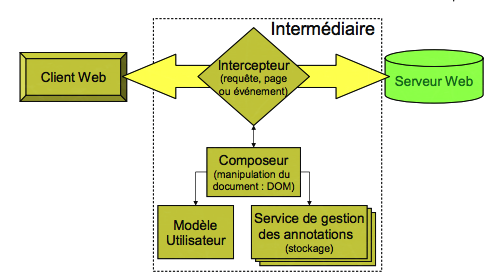
\includegraphics[width=11cm]{AnnotationSys.png}
\caption{Système de notation d'intermédiaire}
\end{figure}
\subparagraph{}
L'annotation sémantique faite référence à plusieurs types distincts d'annotations formelles, explicites et permanentes. Il existe des outils d'annotation basés sur les ontologies {\it Ontology based annotation tool}
et des critères relatifs aux annotations, par exemple : les types de ressources concernées, la structuration des schémas de description, l'automatisation marquée de la mise en place, etc.
\begin{figure}[H]
\centering
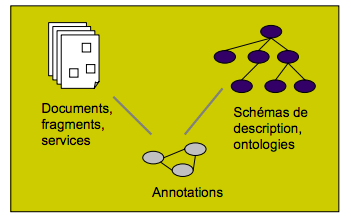
\includegraphics[width=9cm]{diffConnaissances.png}
\caption{Différents niveaux de connaissances}
\end{figure}
\subparagraph{}
L'annotation d'un triplet RDF est une façon d'ajouter des metadonnées à ce triplet pour décrire une restriction spatiale.
\newline
\textit{Comment on utilise les annotations temporelles ?} Un exemple d'utilisation est sur la plateforme ``sig.ma''\footnote{http://sig.ma/} crée par l'institut de recherche irlandais \textit{the digital enterprise research institute in Ireland (DERI)} spécialisé dans le domaine du Web sémantique et les données liées. La plateforme fournit un moteur de recherche par mot clé qui permet de récupérer des images et des textes accessibles par des annotations RDF, ainsi qu'une liste d'URI correspondant à la clé de recherche et des liens vers des ressources Web contenant des données RDF pertinentes.
\section{Analyse des Besoins}
\paragraph{}
Le large succès de Wikipedia (qui est le 2ème site le plus visité sur internet) et le progrès des techniques d’extraction des données ont abouti à la naissance de la construction automatique  de larges bases de connaissances comme DBpedia, YAGO, etc...
\begin{figure}[H]
\centering
\includegraphics[width=10cm]{Sources.png}
\caption{Différentes sources d'informations dans DBpedia depuis Wikipédia et Wikidata}
\end{figure}
\subparagraph{}
Beaucoup de connaissances sont construites en se basant sur l’extraction automatique des faits relationnels dans un texte.
En effet, les bases de connaissances convergent sur les faits statiques et ne donnent pas une grande importance à la dimension temporelle de ces triplets.
En dépit du fait que la majorité des faits évoluent avec le temps, ou ne sont valides que dans une période temporelle précise. Ainsi, nous remarquons que le temps a une dimension significative dans ces bases de connaissances.
\subparagraph{}
La dimension temporelle est particulièrement importante dans les relations binaires comme $isPresidentOf$, $isCEOof$, $isMarriedTo$. Une base de connaissances contenant plusieurs présidents des États-Unis ne peut être consistante que lorsqu’on ajoute une dimension temporelle à ces faits. De plus l’annotation temporelle aide à faire la distinction entre les faits courants et les faits dépassés.
Par exemple le fait ``Kennedy est le président des États-Unis'' est correct, mais n'est plus valide.
Lorsqu’on attache une annotation temporelle à un fait comme celui là, il devient universellement valide.

\section{Problèmatique}
\paragraph{}
Lorsqu’on explore DBpedia, on trouve beaucoup de triplets qui décrivent des informations temporelles. Ces triplets sont généralement liés à un contexte événementiel précis.
Il est plus difficile d’exploiter ces informations si elles ne possèdent pas une structure universellement valide, claire et lisible par la machine. Dans DBpedia, il se trouve que des informations liées au même contexte temporel sont exprimées de la manière suivante : 
\begin{figure}[H]
        \centering
                \centering
                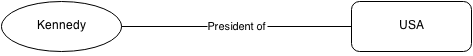
\includegraphics[width=10cm]{ken.png}
               \caption{triplet ''Kennedy''}

\end{figure}
\subparagraph{}
Le premier triplet n'a pas une sémantique valide que en tenant compte du triplet suivant~: 
\begin{figure}[H]
        \centering
                \centering
                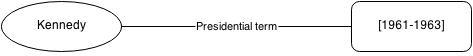
\includegraphics[width=10cm]{presidterm.png}
               \caption{triplet presidential term ''Kennedy''}

\end{figure}
\subparagraph{}
Dans cette étude, on vise plutôt à annoter les triplets ($s$, $p$, $o$) avec une étiquette temporelle qui indique et précise la validité de ce terme dans un cadre logique qui appartient au monde réel où en dehors de ce cadre, on peut dire que ce triplet RDF n’est pas valide et qu’on ne peut pas l’utiliser.

\section{Étude préliminaire et approches possibles}
\subsection{Web Collaboratif}
\paragraph{}
C'est le Web qui s'appuie sur les utilisateurs pour construire son contenu. Nous avons commencé notre travail de recherche par une étude préliminaire autour du contenu de ces plateformes collaboratives. Aussi, nous avons étudié les pistes possibles pour l'exploitation des dumps de Wikipédia et Wikidata. Tout d'abord, nous avons téléchargé les fichiers des collections XML et nous avons observé la structure des informations dans ces sources d'informations. Ensuite nous avons implémenté un premier algorithme d'extraction en utilisant un parseur XML (SAX\footnote{http://fr.wikipedia.org/wiki/Simple\_API\_for\_XML}).
La figure ci-dessous représente notre schéma de modélisation dans lequel nous avons procédé avec une modélisation qui touche directement la source principale d'informations Wikipédia.
\begin{figure}[H]
        \centering
                \centering
                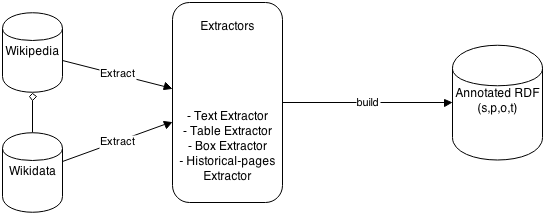
\includegraphics[width=13cm]{modelisation.png}
               \caption{Première approche : schéma de modélisation générale}

\end{figure}
\subparagraph{}
Cette modélisation est une première rubrique d'analyse et de conception d'une solution qui touche les besoins préliminaires de notre étude. Par ailleurs, nous avons retrouvé une autre modélisation plus proche à nos besoins principaux et que nous vous détaillerons par la suite.
\subsection{Usage du traitement automatique des langues}
\paragraph{}
Le traitement automatique de la langue (TAL) est une discipline à la frontière de la linguistique, qui est intimement liée à l'intelligence artificielle.
On distingue plusieurs domaines d'application de TAL comme la traduction automatique, la génération automatique de texte, la correction orthographique, la reconnaissance de l'écriture manuscrite, etc...
Dans le cadre des annotations temporelles on pourrait utiliser les TAL pour :

\paragraph{}
{\it Ambiguïtés temporelles}, est la propriété d'un mot ou d'une suite de mots (comme dans notre cas) qui peuvent avoir un ou plusieurs sens d'analyses grammaticales possibles. Dans une phrase simple ou composée, l'indicateur temporel peut avoir plusieurs sens tout dépend du contexte de la phrase. Les informations temporelles peuvent avoir des représentations différentes~: 
\begin{itemize}
\item Un évènement ``Je vous propose un rendez-vous $demain$ pour parler de ma plateforme PiSharing''. \item Une connaissance ``Jacques Chirac est le président de la république Française'' \textbf{ mais quand ?}.
\end{itemize}

\subparagraph{} 
Le présent par exemple peut avoir plusieurs sens ou contextes : présent de narration, présent de généralité, présent qui réfère au futur proche, etc...
Les signaux temporels sont ambigus par exemple dans ces expressions : il court pour rattraper le temps, tu tournes après la rivière, etc… On remarque qu'il y a des indicateurs temporels, mais ce n'est pas le temps qui est relatif à un événement qui peut nous intéresser.
\paragraph{}
La plupart des expressions sont floues comme: il y a deux ans, chaque deux semaines, j’arrive dans deux secondes, etc... En effet, il n'y a pas une logique descriptive qui peut nous aider à mettre un le lien entre l'événement et la période temporelle. L’analyse du temps s’inscrit dans la compréhension globale des textes, et des évènements auxquels on fait référence dans ce texte non pas en analysant une phrase comme suit. 
\newline
Modalité~: ``l’équipe de France voulait gagner la coupe du monde en 2014.'' 
\newline
Anaphore~:  ``..., cela pourrait avoir lieu dans les éditions suivantes.''
\subparagraph{}
Les évènements décrits (et que l’on souhaite fixer temporellement) peuvent être : duratifs ou ponctuels/accomplis ou inaccomplis. 
De même pour les dates qui peuvent être des dates absolues ``le 18 mars, c'est mon anniversaire'' ; ou bien des dates relatives par rapport au moment de l’énonciation par exemple : ``il y a deux ans''. Pour la durée aussi on distingue plusieurs types comme la durée absolue ``durant 2 ans'' et la durée relative ``depuis un an''. Dans un texte, on trouve aussi un ensemble d'expressions de fréquence comme ``tous les ans, le vendredi 13'' et des expressions plus complexes comme ``après la Révolution Tunisienne''.
\subparagraph{}
Les textes contiennent des informations temporelles de taille massive qui sont difficilement exploitables. Nous avons donné une vue globale sur cette procédure que nous avons décidé de ne pas l'adopter parce que notre objectif est d'annoter des triplets RDF plutôt que de faire l'analyse des textes.
\paragraph{}
{\it Exploration des historiques des modifications dans Wikipédia}, l'historique est une page attachée à un article encyclopédique pour conserver le journal de la plupart des modifications qui ont été apportées à cet article. Cette page permet de connaître la date, l'auteur et la teneur externe de chaque modification.
Dans cette encyclopédie, nous avons remarqué qu'à partir de l'historique de modifications, on peut déduire plusieurs informations liées à deux ou plusieurs contextes temporels différents.
Nous souhaitons, si c’est possible, extraire ces informations temporelles et les rendre exploitables dans DBpedia.
\begin{figure}[H]
\centering
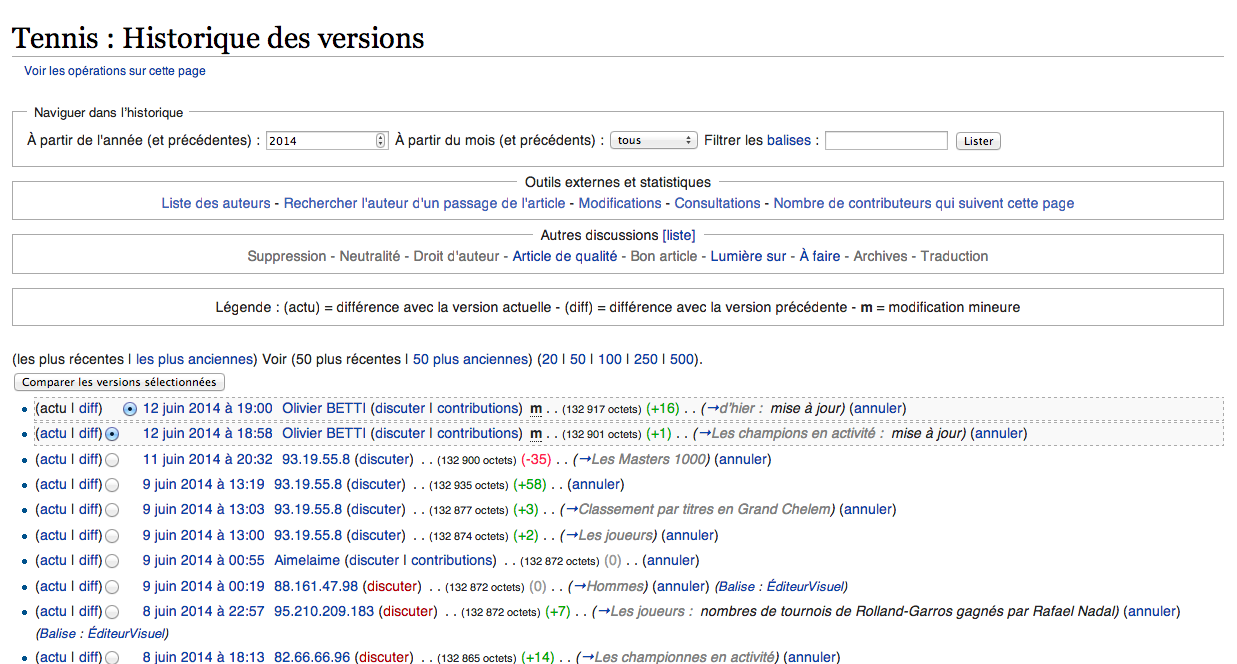
\includegraphics[width=14cm]{NEWHISTORIQUE.png}
\caption{Historique d'articles Wikipédia}
\end{figure}
\subparagraph{}
Cette partie impose une petite partie de TAL et ne peut s'appliquer que sur des faits récentes.
\newpage
\section{Architecture d'extraction de DBpedia}
\paragraph{}
DBpedia est un travail de recherche communautaire, cette base de connaissances décrit plus que $3.4$ millions d'entité. DBpedia définit un identifiant global et unique qui peut être déréférencé sur le Web dans une riche description RDF de l'entité, des définitions et descriptions lisibles dans $119$ langues, la relation avec d'autres ressources, la classification à quatre hiérarchies de concepts, des faits divers liées à d'autres sources de données sur le Web. Ce qui permet à DBpedia d'être un pôle central d'interconnexion pour le Web de données émergent.   
\subsection{Vue d'ensemble du framework d'extraction DBpedia}
\begin{figure}[H]
\centering
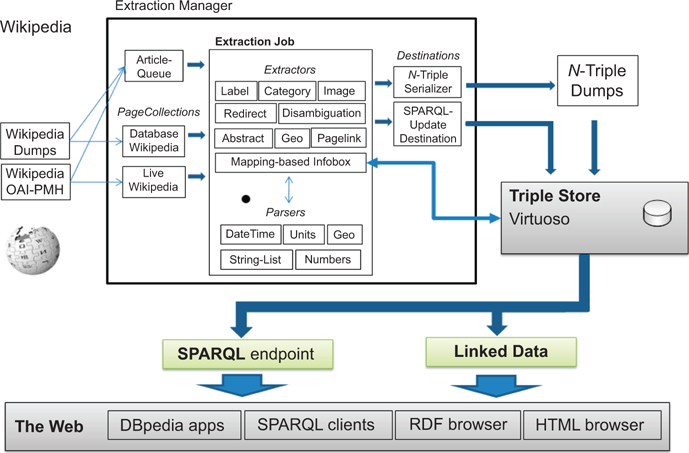
\includegraphics[width=12cm]{dbpediaExtra.png}
\caption{Extracteur DBpedia}
\end{figure}
La figure ci-dessus montre l'architecture du système d'extraction des connaissances dans DBpedia.
D'apres Morsey et al~\cite{morsey2012} les principaux éléments du système sont les suivants : $PageCollections$ est une abstraction des ressources locales ou distantes des articles de Wikipédia, $Collections$ stokent ou sérialisent les triplets RDF extraites, $Extractors$ qui transforme un type spécifique de la syntaxe wiki en triplet, $Parsers$ soutiennent les $Extractors$ en déterminant les types de données, convertit les valeurs entre différentes unités et fractionne les marqueurs dans des listes. L'$Extraction$ $Job$ regroupe une collection de pages, extracteurs et destination dans le flux de travail $workflow$.
Le noyau de ce système est l'$Extraction$ $Manager$ qui gère le processus  d'adoption des articles de Wikipédia sur les $Extractors$ et donne les résultats à la destination.
Le gestionnaire d'extraction $Extraction$ $Manager$ gère également la gestion des URI et résoud les redirections entre les articles : ce système se compose de $11$ extracteurs qui traitent les types des contenus de Wikipédia {\tt(Labels, Abstracts, Interlanguage links, Images, Redirects, Disambiguation,
External Links, Pagelinks,}
\newline
{\tt Homepages, Categories, Geo-coordinates)}.
Ce framework d'extraction DBpedia est mise en place pour réaliser deux flux : extraction à partir des sources de données {\tt(DataBaseWikipedia page collections)} et une procédure d'extraction directe
{\tt(LiveWikipedia page collections with the OAI-PMH protocol)} pour obtenir la version courante des articles. Notre point d'accès à ce système d'extraction, plus précisément à la base RDF {\tt Triple Strore} sera à travers des requêtes SPARQL. 
\subsection{Notre proposition}
\paragraph{}
En analysant les $dumps$ DBpedia et en observant l'architecture de cette base de connaissance, nous avons remarqué que pour annoter temporellement les triplets RDF de DBpedia il est plus intéressant d'extraire l'ensemble des propriétés dans DBpedia, puis de trouver des faits qui ont un trait avec le temps, donner une liste de couples à partir de laquelle un expert choisit un couple et valide les résultats de notre algorithme.
\subsection{Modélisation}
\paragraph{}
Le modèle quaternaire est un modèle qui extrait la base RDF d'un fait précis et assi le fait rattaché au premier ayant une dimension temporelle. Les deux exemples suivant montrent le principe de ce modèle.
\paragraph{}
{\it <politician> elected <president of US> on <date>}
\newline
f1, Kennedy elected PresidentOf USA 
\newline
f2:f1, HappenedDate, $HappenedDate$ est utilisée pour dire que le fait est valide que dans ce point du temps.
\paragraph{}
{\it <politician> served as <politician office> from <date> to <date>}
\newline
f1, Kennedy holdsPoliticalPosition PresidentOf USA 
\newline
f2:f1, startedOnDate 
\newline
f3:f1, endedOnDate

\begin{figure}[H]
        \centering
                \centering
                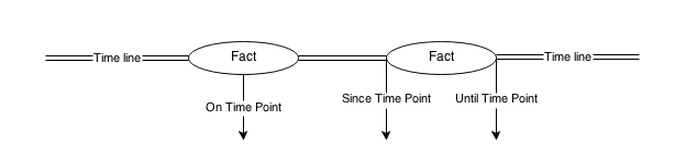
\includegraphics[width=13cm]{timeline.png}
               \caption{Chronologie des événements}

\end{figure}
\subparagraph{}
Ce modèle est capable d'exprimer la validité temporelle d’un triplet RDF d’une manière à la fois intelligente et lisible par la machine ; on souhaite rattacher au triplet valide que dans un point du temps ou une plage temporelle bien précise sous la frome d'une étiquette temporelle adéquate comme le montre la figure suivante.
\begin{figure}[H]
        \centering
                \centering
                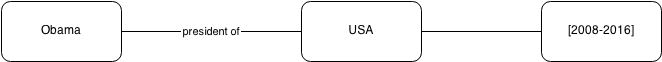
\includegraphics[width=13cm]{obamaQuad.png}
               \caption{Modélisation quadruplet}

\end{figure}
\subparagraph{}
On s'intéresse particulièrement au format N-Quads comme format de sortie de notre algorithme. Les quadruplets vont être formalisés de la manière suivante~:
\subparagraph{}
$<s,p,o,t>$ : un sujet, prédicat, objet avec un point de temps.
\subparagraph{}
$<s,p,o,[t1,t2]>$ : de même avec une intervalle de temps.
\subsection{Notre hypothèse}
\paragraph{}
Après une observation approfondie dans les sources de données dans DBpédia, nous avons repéré des relations logiques entre des propriétés comme \{($firstAssentPerson$, $firstAssentYear$) ou ($beatifiedBy$, $beatifiedDate$)\}. Nous avons trouvé plusieurs propriétés qui ont un lien logique entre eux, les relations temporelles ont comme objet un point du temps particulier et partagent le même sujet ou la même ressource avec une autre propriété.
\newpage
\subparagraph{}
Durant cette étude nous avons essayé de valider cette hypothèse :
\begin{verbatim}
if (x propTemp t) and (x propWithToken z) then
             (x propWithToken z) t 
\end{verbatim}

\begin{itemize}
\item $propTemp$ est une propriété DBpédia dont le nom contient une indication temporelle.(Year, Date).
\item $propWithToken$ est une propriété DBpédia avec un nom qui le même motif.
\end{itemize}
$t$ est l'annotation temporelle du triplet ($x$,$propWithToken$,$z$).

\subparagraph{}
Nous avons présenté cette hypothèse sous forme d'une requête SPARQL. Cette requête interroge l'ensemble des ressources sur DBpédia et retourne des résultats si c'est possible.
Notre hypothèse porte principalement sur le fait d'annoté temporellement les ressources de DBpedia en utilisant en essayant de repérer deux triplets portent sur un même sujet et permettant à les relier dont le but est d'avoir un quadruplet valide. La liste des couples ($PropTemp$, $PropWithToken$)
est donnée comme sortie d'une procédure d'extraction intelligente de l'ensemble des propriétés de DBpédia. Toutefois, cette hypothèse n'est pas automatique, elle nécessite un validation de la part d'un expert.
\newpage
\section{Notre choix}
\subsection{Architecture du système}
 \begin{figure}[H]
        \centering
                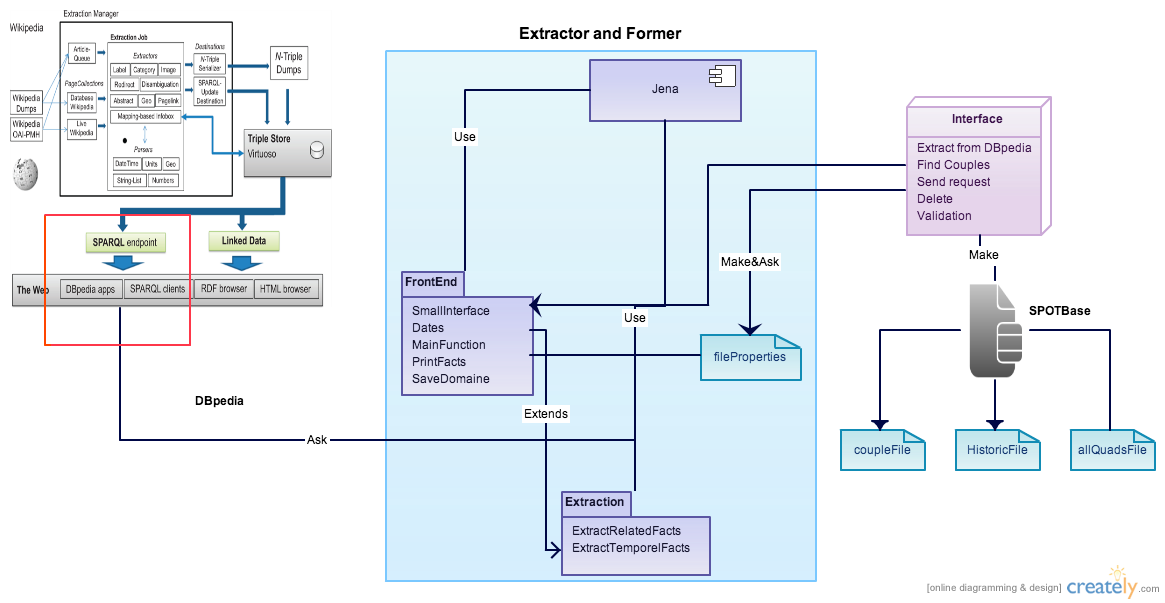
\includegraphics[width=16cm]{NEWArchitecture.png}
               \caption{Architecture de l'application}
\end{figure}
\paragraph{}
L'architecture de notre application se repose principalement sur celle de DBpédia. En premier lieu, nous interrogeons DBpédia pour avoir une liste de propriétés. En effet, nous pouvons prendre la liste de toutes les propriétés en interrogant DBpedia avec $Virtuoso$ $SPARQL$ $Query$ $Editor$\footnote{http://dbpedia.org/sparql}  à l'aide de la requête \begin{verbatim} select distinct ?P where {?S ?P ?O},\end{verbatim}mais on se limite aux propriétés de DBpedia qui ont la forme suivante \begin{verbatim} ?S rdfs:domain ?O \end{verbatim} $rdfs:domain$ est une instance de $rdfs:Property$ qui est utilisé pour indiquer que toute ressource qui possède une propriété donnée est une instance d'une ou plusieurs classes. Le triplet précédant indique que, $S$ est une instance de la classe $rdf:Property$, $O$ est une instance de la classe $rdfs:Class$ et les ressources désignées par les sujets des triplets dont le prédicat est $S$ sont des instances de la classe $O$. Lorsque une propriété $S$ a plus d'une propriété $rdfs:domain$, les ressources indiquées par les sujets des triplets avec prédicat $S$ sont des instances de toutes les classes indiquées par les propriétés $rdfs:domain$. $rdfs:domain$ peut être appliqués à lui-même. $rdfs:domain$ de $rdfs:domain$ est la classe $rdfs:Property$. Cela veut dire que toute ressource avec une propriété $rdfs:domain$ est une instance de $rdf:Property$. 
\subparagraph{}
Ensuite, nous avons choisi de stocker l'ensemble de propriétés dans un fichier pour ne pas avoir des contraintes de mémoire (stockage dans la mémoire vive) et pour ne pas interroger la base de connaissances à chaque fois. Cette procédure se fait une seule fois lors du premier lancement de l'application et elle ne sera plus nécessaire après, car il suffit de spécifier le nom du fichier des propriétés DBpédia que nous avons utilisé l'hors de la première exécution, mais nous avons mis la possibilité d'extraction et mise à jour de ce fichier parce qu'il se trouve que DBpédia change quotidiennement et il y a des propriétés qui s'ajoutent au fur et à mesure à cette base de connaissance. Puis, à partir de ces propriétés, nous avons implémenté un algorithme d'extraction qui produit en sortie une liste de couples de propriétés (PropriétéTemporelle, PropriétéReliée). Dans l'application, nous avons choisi de prendre l'avis d'un expert pour valider les résultats de notre algorithme à travers une liste labellisée d'une partie des quadruplets que nous avons réussi à former et à extraire automatiquement dans un $output$ $Textarea$. Nous avons écrit notre hypothèse de base sous forme d'une requête SPARQL de la manière suivante :
\begin{verbatim}
PREFIX rdfs: <http://www.w3.org/2000/01/rdf-schema#> 
PREFIX dbp:<http://dbpedia.org/ontology/> 
SELECT CONCAT(?label1, relatedProp , ?label2, ' : ', ?date) 
			WHERE {  
					 ?S   		dbp:relatedProp 	 ?O;
							dbp:tempProp		 ?date;
							rdfs:label 			 ?label1.
					?O 		rdfs:label ?label2.
					FILTER(lang(?label1)='en' && lang(?label2)='en'}
\end{verbatim}
{\it - tempProp est une propriété temporelle proposé.}
\newline
{\it - relatedProp est une propriété reliée à tempProp partage avec elle un même motif ``Token''.}
\subparagraph{}
L'objectif de cette procédure est de permettre à l'expert de valider ou ne pas valider la logique de la représentation des quadruplets. Enfin, la validation des résultats permet de stocker l'ensemble des résultats (triplets annotés) dans un fichier portant les labels du couple et un autre fichier ``allQuadsFile'' contenant tous les quadruplets validés. Par la suite, notre sauvegarde se fait automatiquement dans le fichier CSV d'historique qui a forme suivante :
\newline
{\tt (attribute,tempAttribute,boolean,exploration\_Date,keep,file)} 
\begin{itemize}
\item $attribute$ et $tempAttribute$ représentent le couple de propriétés DBpédia.
\item $boolean$ peut être $0$ ou $1$ qui désignent respectivement la volonté de l'expert de valider ou ne pas validé les résultats.
\item $exploration\_Date$ est la date de l'exploration
\item $keep$ représente le nombre de quadruplets que nous avons formé à partir d'un couple de propriétés.
\item $file$ est le nom de fichier dans lequel nous avons stocké les résultats (Quads).
\end{itemize}
\subparagraph{}
Ce fichier nous permet d'avoir une vision globale sur les résultats de notre étude.
L'ensemble de fichiers seront stockés dans un dossier forment une base de données de sortie que nous avons appelé $SPOTBase$.
\subsection{Analyse et discussion}
\paragraph{}
Nous avons réussi à former $305$ couples de propriétés, et nous pouvons encore restreindre ce nombre. Dans notre méthode, nous avons choisi d'extraire même les propriétés reliées aux propriétés temporelles qui contiennent un motif similaire et non pas seulement qui sont identique au suffixe d'une propriété temporelle. Cela a été dans la mesure d'augmenter le nombre des couples de propriétés de test pour avoir une vision globale sur l'efficacité de notre système, d'avoir plus de possibilités et d'analyser par la suite les différents résultats. 
\subparagraph{}
Avec certains couples, nous avons eu des très bons résultats, par exemple avec le couple ($deathCause$,$deathYear$) nous avons réussi à formé $2766$ quads. La figure ci-dessous montre le format de la sortie de notre algorithme.
 \begin{figure}[H]
        \centering
                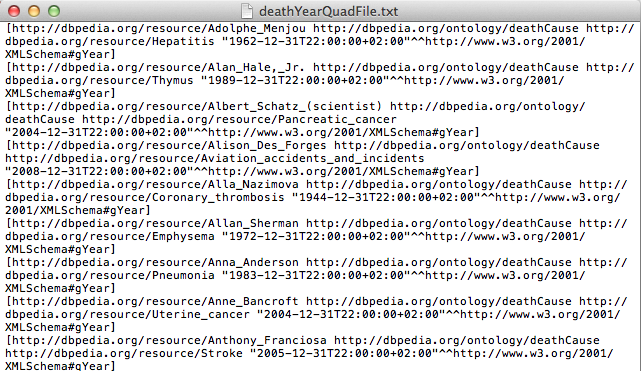
\includegraphics[width=13cm]{DeathYearCause.png}
               \caption{Fichier de Quadruplet DeathYear et DeathCause}
\end{figure}
\subparagraph{}
Il se trouve aussi qu'il y a des couples qui valident notre hypothèse mais qui ne donnent pas de résultats. Il se peut que les deux triplets ne partagent pas le même sujet comme \{(wineRegion, wineYear),(whaDraft, whaDraftYear),(areaCode, areaDate), etc...\}
\section{Outils de développement}
\subsection{ Java}
\paragraph{}
Le choix de développer le logiciel sous forme d'une application $Java$ était un choix personnel et qui s'explique de nombreuses manières. Premièrement, la maîtrise de ce langage de programmation me permet d'utiliser des différentes structures de données et d'explorer la documentation de certaines méthodes plus facilement. De plus, il existe plusieurs sources de documentation sur le Web. En outre une large communauté aide à répondre aux questions si jamais on rencontre des difficultés. Il existe une version Java de DBpédia et cela permet plus facilement d'intégrer mon application open source et disponible sur mon compte\footnote{https://github.com/metanote/Extraction} github. Enfin, nous avons utilisé les librairies $Jena$ qui sont aussi écrites en Java. 
\subsection{Jena}
Jena\footnote{https://jena.apache.org/} est un $Framework$ open source écrit en Java pour construire des applications dans les domaines du
$LinkedData$ et le Web sémantique. Nous avons utilisé les différentes librairies des ce $Framework$ pour interroger DBpédia avec des requêtes SPARQL. $Jena$ est composé de plusieurs programmes différents qui interagissent entre eux pour traiter des données écrites en RDF. $Jena$ fournit un support pour le langage de définition d'ontologies (OWL). Ce $Framework$ se compose des différentes API RDF, Ontology et SPARQL. Une couche interface d'application et une troisième couche pour le stockage. La figure ci-dessous présente en détaille les différentes composantes de Jena.
 \begin{figure}[H]
        \centering
                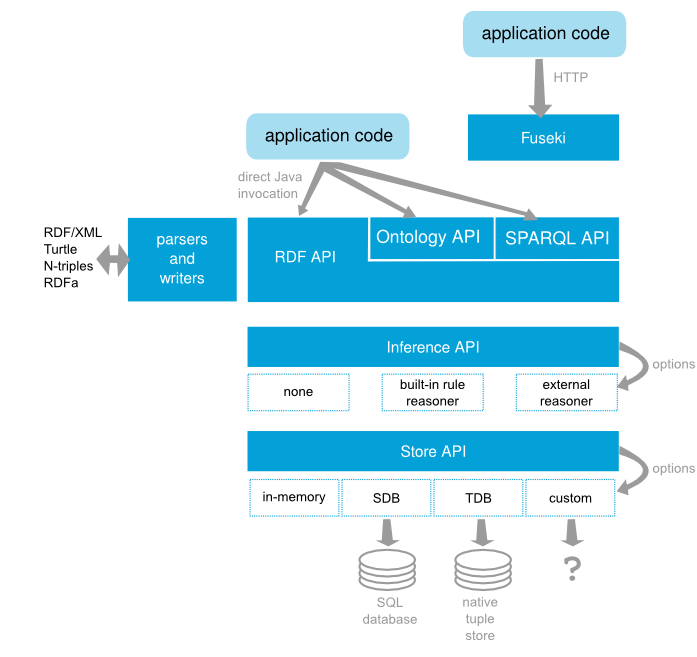
\includegraphics[width=12cm]{Jena.png}
               \caption{Jena Interaction entre les différents API}
\end{figure}
\subsection{Résultats et Validation}
\paragraph{}
Durant cette étude, nous avons essayé d'annoter temporellement des triplets DBpedia. Nous avons réussi à former automatiquement un nombre important de quadruplets à partir de couples de propriétés qui valident notre hypthèse. Pour certaines propriétés, notre programme prend une quinzaine de minutes des parfois pour extraire des triplets depuis la base DBpedia. Sachant qu'on utilise une machine sous OS x avec un processeur $2$ GHz Intel Core i$7$ er $8$ GO de mémoire. Cela est dû au nombre gigantesque de quadruplets qu'on obtient, parmis nos meilleurs résultat celle du couple de propriétés (BirthPlace, BirthDate) donnent $50000$ triplets annotés.
\subparagraph{}
Nous avons stocké plus que $106998$ quads que nous avons réussi à former dans le fichier $AllQaudsFile$. Nous avons remarqué que certains couples valident bien notre hypothèse et donne des excellents résultats. Certes, il y a d'autres couples ne donnent aucun résultat. Le problème, c'est que toutes les propriétés DBpédia ne suivent pas toujours la même logique de représentation. Si tel n'était pas le cas, nous pouvons avoir beaucoup plus de résultats.
Dans le Web sémantique, nous avons remarqué qu'il est très important de mettre des conventions pour la représentation des données. Cela permet non seulement d'utiliser les triplets existants, mais aussi de mettre des hypothèses permettant de construire des travaux au dessus de ce qui existait. Le Web sémantique évolue s'il se repose sur une structure de métadonnées générique, claire et réutilisable. Dans cette étude, nous avons traité des triplets DBpédia. Nous avons réussi à implémenter une solution pour annoter des triplets qui ont un trait avec le temps et nous avons mis ces triplets sous la forme quadruplet. Nous avons manipulé une partie de triplets de la base de données d'entrer pour construire notre base de données quadruplets de sortie que nous avons appelé SPOTBase.

\chapter{Conclusion et perspectives}
\paragraph{}
Comme toute étude de recherche, les portes sont toujours ouvertes pour des améliorations et des adaptations. Notre logiciel est disponible sur le gestionnaire de version GitHub en version open source sur mon compte\footnote{https://github.com/metanote/Extraction} ce qui permet d'ouvrir les pistes à d'autres personnes pour l'utiliser et l'améliorer. 
\section*{Améliorations possibles}
\paragraph{}
Ce logiciel est un outil d'extraction de propriétés à partir de DBpédia, permet de fusionner deux triplets et de les transformer en quadruplets ou autrement des triplets annotés temporellement. Actuellement, cet outil dépend de l'avis d'un expert pour valider les résultats de notre algorithme. Il serait intéressant de rendre toute cette procédure de modélisation automatique. Aussi, on peut intégrer une procédure d'apprentissage, en cherchant à classifier les propriétés DBpédia sous forme de deux classes par exemple (PropWithResult, PropWithoutResult) avec un algorithme d'apprentissage automatique comme (SVM, Adaboost) et en trouvant d'autres motifs pour les couples de propriétés. Dans cette étude, nous avons travaillé avec deux indices temporels (Date, Year). Nous pouvons chercher d'autres indices qui peuvent nous aider à repérer plus de propriétés temporelles dans DBpédia. Nous avons tourné notre algorithme sur $1992$ propriétés DBpédia que nous avons extrait. Il serait intéressant de tourner cet algorithme sur une autre base de faits qui contient plus de faits.
\subparagraph{}
Dans cette application Java, nous avons cherché seulement les propriétés qui dépendent d'un point de temps particulier.
Dans notre hypothèse de base, nous voulons aussi chercher les propriétés qui sont vraies dans un intervalle de temps, des propriétés temporelles comme (MotifStartDate,MotifEndDate), mais dans le fichier de propriétés nous avons repéré $7$ couples de propriétés qui vérifie cette condition. Cela donne seulement $14$ propriétés sur $1992$.
\subparagraph{}
La procédure de la fouille est intéressante pour une quantité de données de masse. Nous avons formé avec les motifs temporels (Year, Date) $305$ couples de propriétés à partir de $1992$ propriétés. Sur les $20$ première couple de propriétés nous avons trouvé $4$ qui donnent des quadruplets valides. Avec une parcours aléatoire de la liste de couple. Nous avons inséré $35$ fichiers de triplets annotés dans le fichier $historic.csv$.
\paragraph{}
Une autre alternative possible se présente comme suit, nous pouvons chercher que les triplets qu'on veut annoter dans DBpédia, puis à partir des faits trouver, il est possible de chercher leurs cadres temporels dans les dumps de Wikipédia et Wikidata.
\paragraph{}
Il est intéressent de fusionner deux triplets afin d'avoir un seul plus structuré. La représentation de connaissances nous permet non seulement de les utiliser, mais aussi de faire des déductions à partir de ces données pour exprimer d'autres concepts. Nous avons remarqué aussi que la modélisation des connaissances permet de rendre les informations plus utiles pour les traitements et il peut éviter beaucoup de redondances. Nous savons qu'actuellement on parle plus de l'énorme quantité de données ou les données massives $Big$ $Data$ sur le Web. Derrière ces mots se cachent l’incroyable quantité de données disponible notamment sur le net, et surtout la manière dont on peut les traiter pour obtenir des informations utiles. On se rend compte de la mauvaise gestion, la duplication, la perte de l'information et la difficulté liée à la recherche de ces informations. C'est pour cela, nous cherchons toujours à optimiser l'usage de ces métadonnées et structuré les données sur le Web.
\subparagraph{}
D'après une étude faite par EMC\footnote{http://www.emc.com/leadership/digital-universe/index.htm}{\it the digital universe study with  reasearch and analysis by IDC}, la firme IDC\footnote{http://www.idc.fr/}, mandatée par EMC (spécialiste des logiciels et systèmes de stockage), a réalisé une étude sur la prolifération de ces données et anticipe déjà ce que cela donnera en $2020$. Les résultats sont particulièrement intéressants. Voici les principaux enseignements :
\begin{itemize}
\item En $2011$, $5$ exaoctets de données étaient générés tous les deux jours. Cela se fait désormais en $10$ minutes seulement.
\item Seules $0,5$\% de ces données sont analysées
\item Il n’y avait que $130$ exaoctets de données dans l’univers numérique en $2005$. Il devrait y en avoir plus de $40 000$ à l’horizon $2020$.
\item En $2020$, les données représenteront l’équivalent de plus de $5 000$ GO par personne.
\item En $2012$, $35$\% de ces informations nécessiterait une protection, mais ce n’est le cas que pour $20$\% d’entre elles.
\end{itemize}
\begin{figure}[H]
        \centering
                \centering
                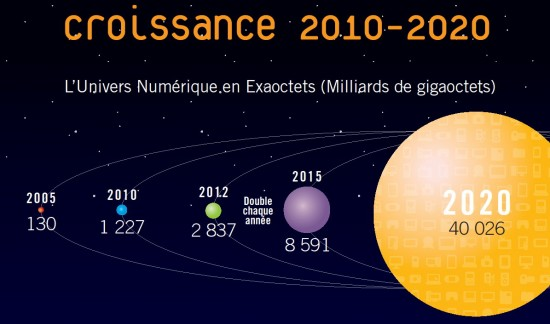
\includegraphics[width=10cm]{datas.jpg}
               \caption{L'univers des données}

\end{figure}
\newpage
\section*{Conclusion}
\paragraph{}
Le stage réalisé a été enrichissant de plusieurs façons. En effet, bien que ce stage soit un stage orienté recherche, il comporte de nombreux aspects d'ingénierie. Les recherches effectuées sont des réponses aux besoins qui ont été accordées dans d'autres travaux de recherche sur l'annotation temporelle et qui est aussi lié aux travaux de mes tuteurs de stage. Les réponses sont également dirigées vers du concret notamment l'élaboration d'une application Java. Cette dualité recherche-ingénierie a été motivante et m'a permis d'affiner une certaine ouverture d'esprit et d'améliorer mes connaissances dans le domaine du Web sémantique.
\subparagraph{}
En plus, durant ce stage, j'ai assisté des présentations dans les domaines du Web sémantique et Big Data. Cela m'a permis de voir les études et les travaux dans ces domaines. La rencontre de différentes visions est toujours intéressante et a permis dans ce cas de situer l'informatique et l'utilisation. Par ailleurs, le travail dans un milieu de recherche m'a permis de chercher des réponses à des questions et résoudre des problématiques intéresantes.
\subparagraph{}
Enfin, l'étude d'annotation temporelle des données DBpédia m'a permis d'apporofondir mes connaissances dans le domaine du Web sémantique et de prendre conscience de son importance. Je suis dorénavant intimement convaincu que les recherches dans le Web sémantique vont permettre d'évoluer le Web et de concrétiser la vision de Tim Berners-Lee.   

\backmatter
\include{Annexes}
\bibliographystyle{alpha}
\bibliography{Biblio.bib} 

\addcontentsline{toc}{chapter}{Bibliographie}
\printglossary[title=Glossaire]
\makeglossaries
\end{document}